\chapter{Project Development}
\begin{figure}[h!]
    \centering
    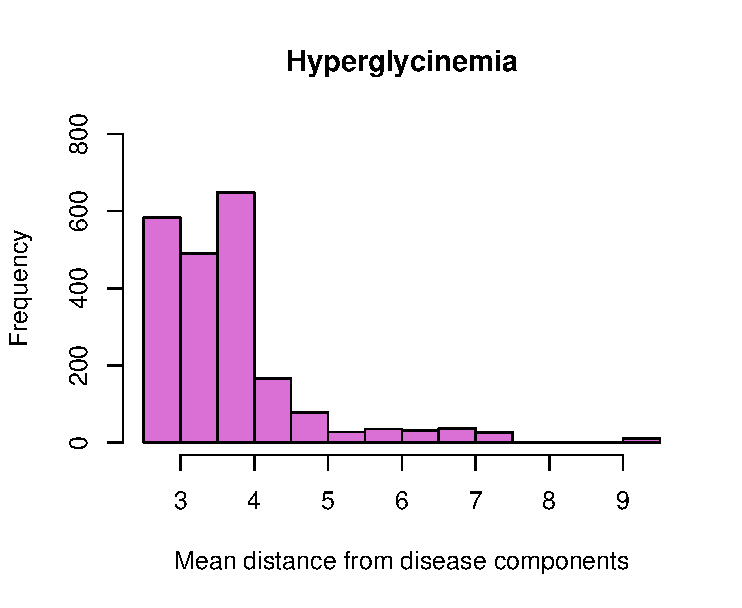
\includegraphics[scale=0.2]{Images/Hyperglycinemia.pdf}
    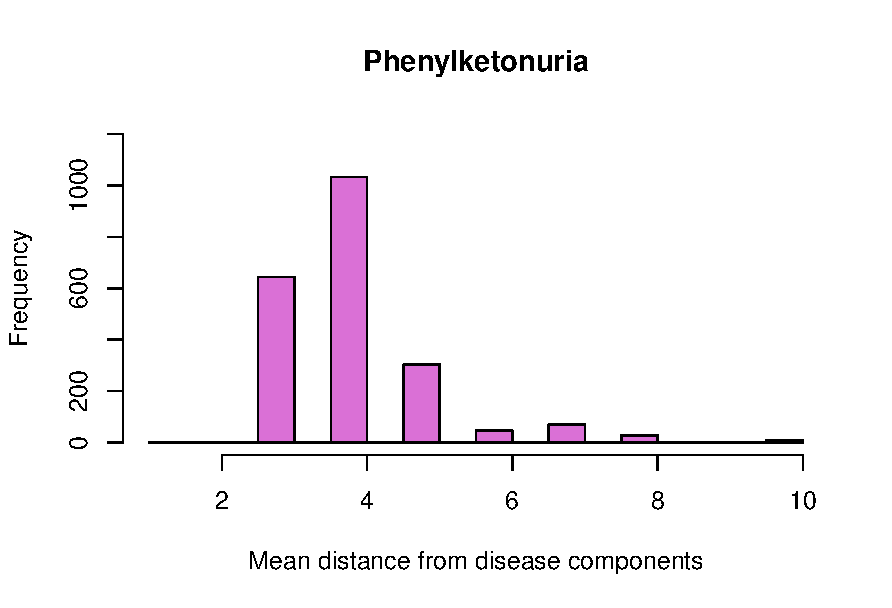
\includegraphics[scale=0.2]{Images/Phenylketonuria.pdf}
    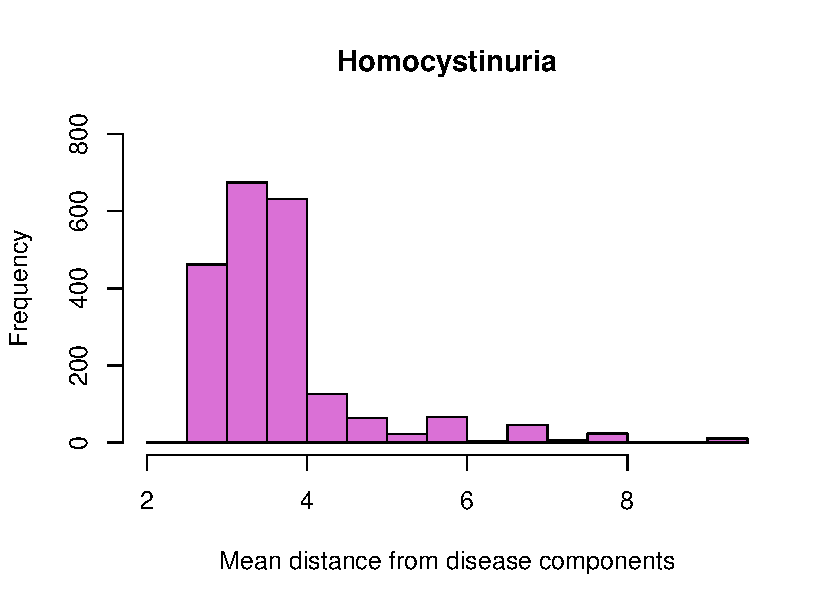
\includegraphics[scale=0.2]{Images/Homocystinuria.pdf}
    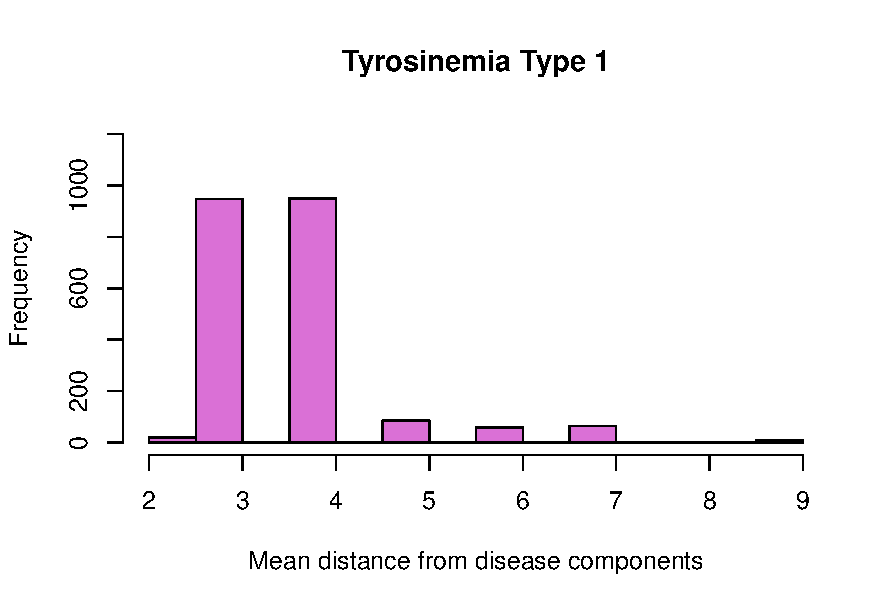
\includegraphics[scale=0.2]{Images/Tyrosinemia Type I.pdf}
    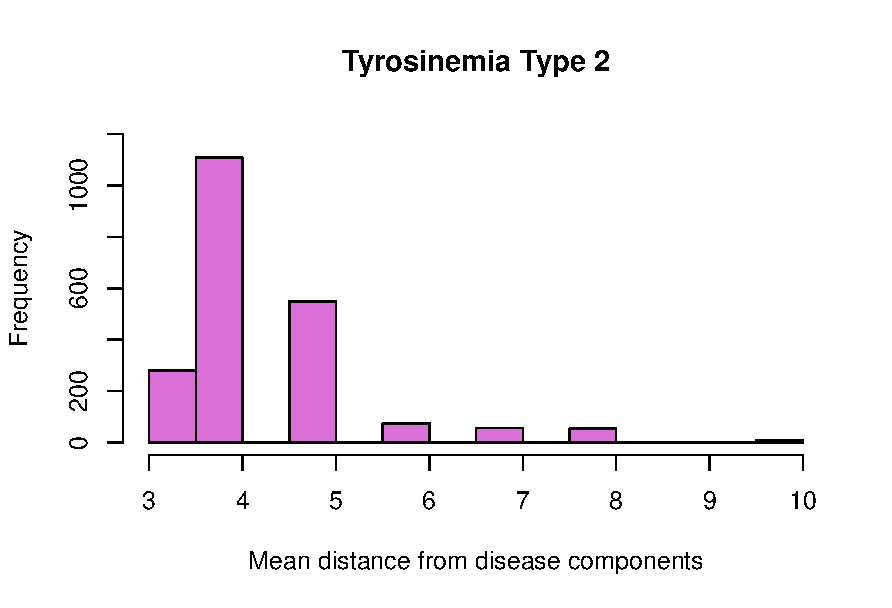
\includegraphics[scale=0.2]{Images/Tyrosinemia Type II.pdf}
    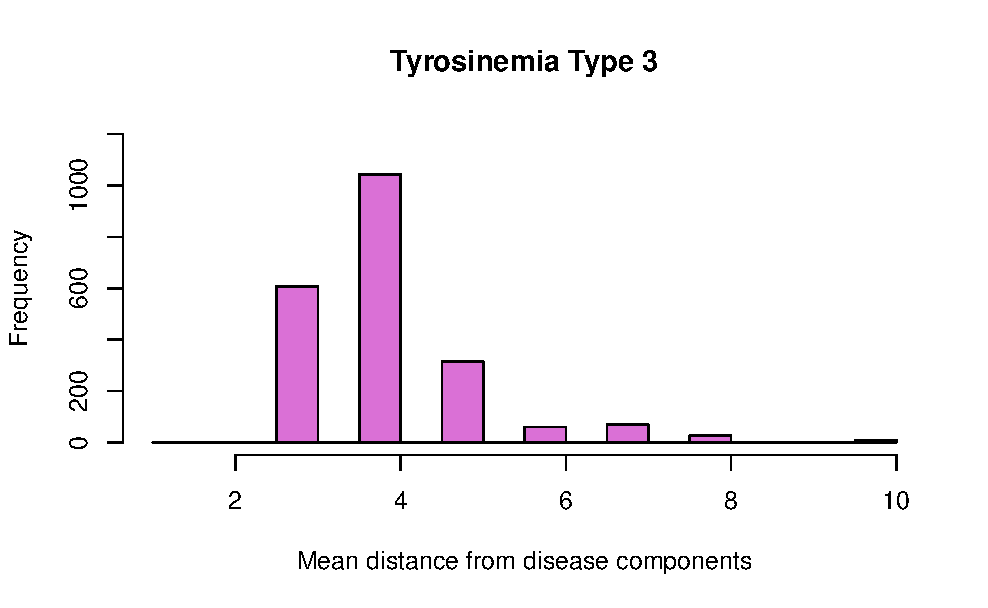
\includegraphics[scale=0.2]{Images/Tyrosinemia Type III.pdf}
    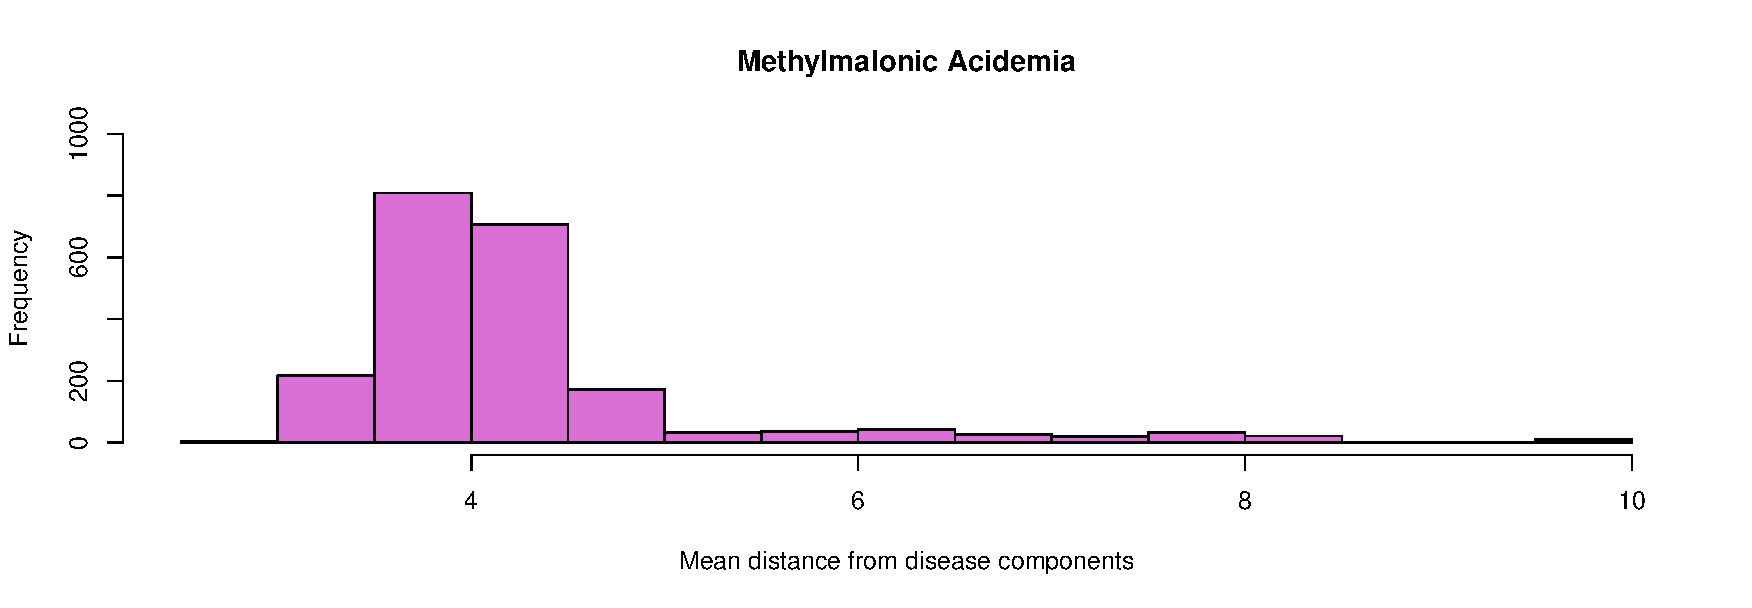
\includegraphics[scale=0.2]{Images/Methylmalonic Acidemia.pdf}
    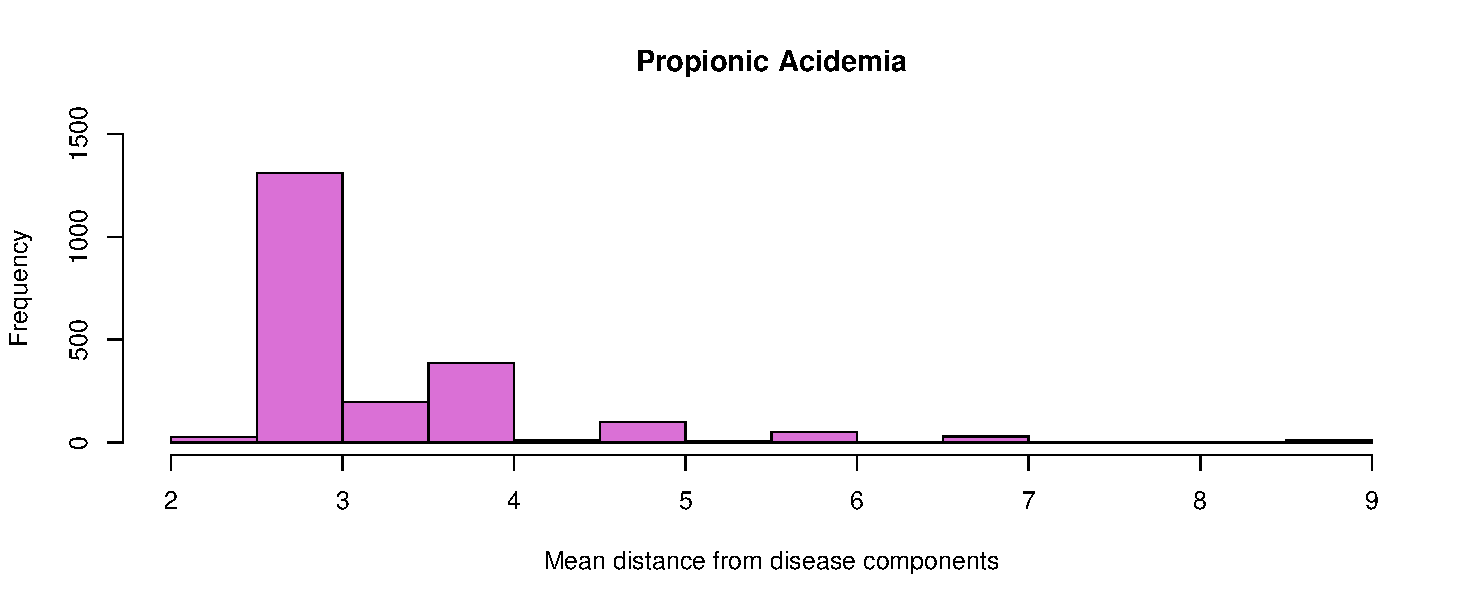
\includegraphics[scale=0.2]{Images/Propionic Acidemia.pdf}
    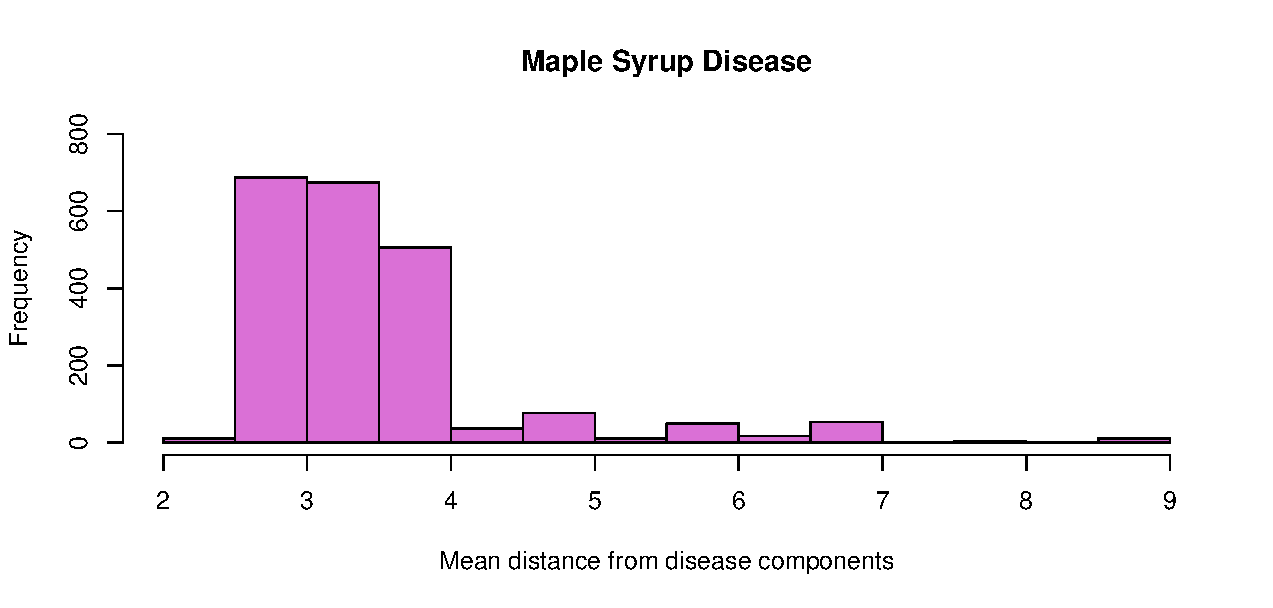
\includegraphics[scale=0.2]{Images/Maple Syrup Disease.pdf}
    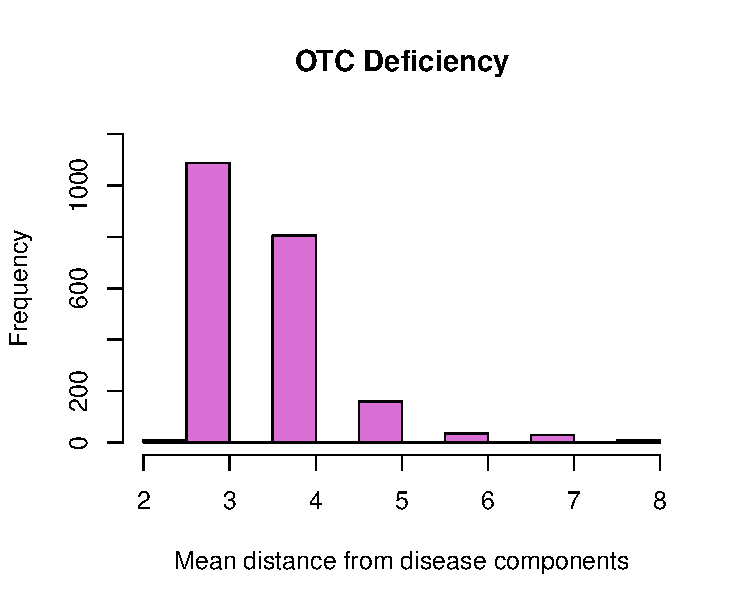
\includegraphics[scale=0.2]{Images/OTC Deficiency.pdf}
    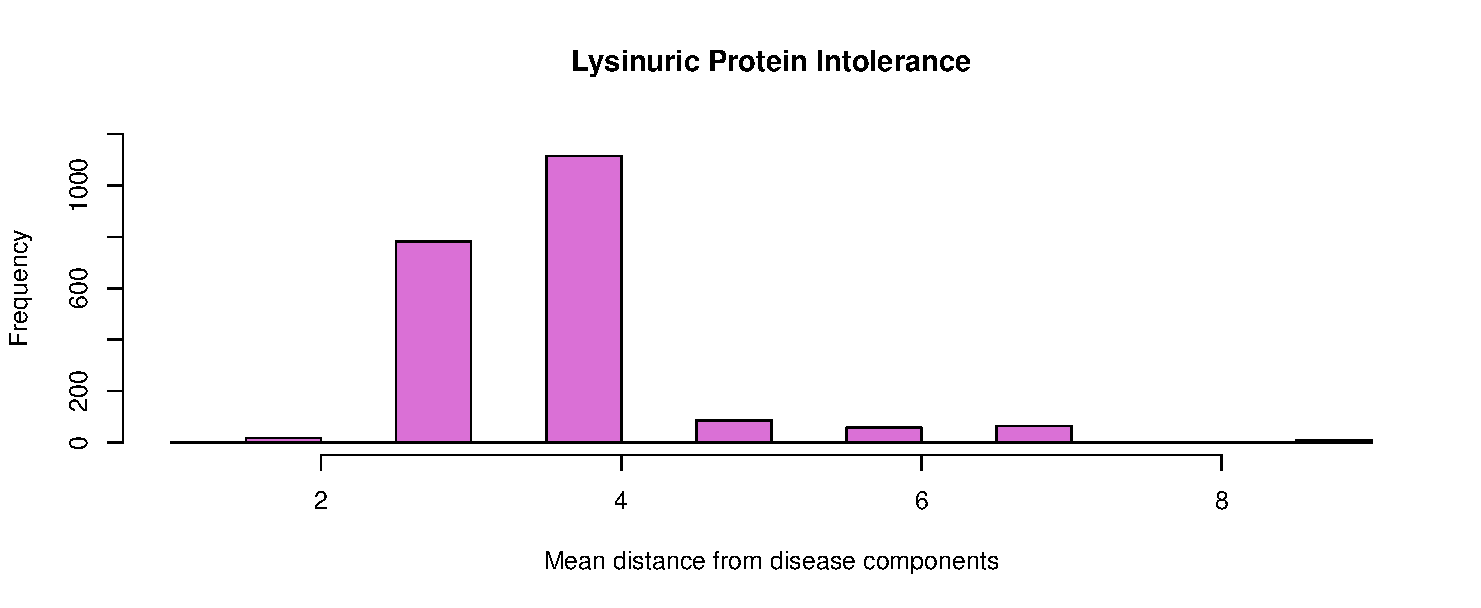
\includegraphics[scale=0.2]{Images/Lisinuric Protein Intolerance.pdf}
    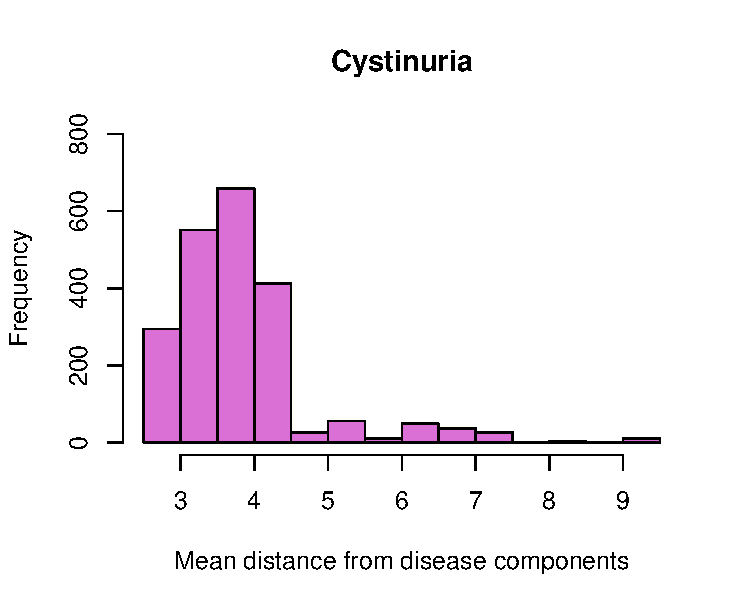
\includegraphics[scale=0.2]{Images/Cystinuria.pdf}
    \caption{Examples}
    \label{fig:results}
\end{figure}
\FloatBarrier